\documentclass[12pt,a4paper,oneside]{report}

% -------------------------------------------------
% Lingua e codifica
% -------------------------------------------------
\usepackage[italian]{babel}
\usepackage[T1]{fontenc}
\usepackage[utf8]{inputenc}

% -------------------------------------------------
% Margini
% -------------------------------------------------
\usepackage[a4paper,margin=2.7cm]{geometry}

% -------------------------------------------------
% Grafica e tabelle
% -------------------------------------------------
\usepackage{graphicx}
\usepackage{float}
\usepackage{booktabs}
\usepackage{array}
\usepackage{caption}
\usepackage{subcaption}

\graphicspath{
  {./images/cap1/}
  {./images/cap2/}
  {./images/cap3/}
  {./images/cap4/}
  {./images/cap5/}
  {./images/cap6/}
  {./images/cap7/}
  {./images/cap8/}
}

% -------------------------------------------------
% Matematica
% -------------------------------------------------
\usepackage{amsmath,amssymb}

% -------------------------------------------------
% Liste personalizzate
% -------------------------------------------------
\usepackage{enumitem}
\setlist{noitemsep}

% -------------------------------------------------
% Codice
% -------------------------------------------------
\usepackage{listings}
\usepackage{xcolor}

\lstset{
  basicstyle=\ttfamily\small,
  breaklines=true,
  frame=single,
  numbers=left,
  numberstyle=\tiny,
  keywordstyle=\color{blue},
  commentstyle=\color{gray},
  stringstyle=\color{orange},
  showstringspaces=false
}

% -------------------------------------------------
% Link
% -------------------------------------------------
\usepackage[hidelinks]{hyperref}

% -------------------------------------------------
% Bibliografia
% -------------------------------------------------
\usepackage[numbers]{natbib}

% -------------------------------------------------
% Frontespizio
% -------------------------------------------------
\usepackage{tikz}
\definecolor{accentblue}{RGB}{0,60,120}

% -------------------------------------------------
% Spaziatura
% -------------------------------------------------
\setlength{\parskip}{0.4em}
\setlength{\parindent}{0pt}

% =================================================
% DOCUMENTO
% =================================================

\begin{document}

% -------------------------------------------------
% Frontespizio
% -------------------------------------------------
\begin{titlepage}
\centering

\vspace*{1.5cm}

{\Huge \textbf{Università degli Studi di Catania}}\\[0.5cm]
{\large Dipartimento di Matematica e Informatica}\\[2cm]

{\Large \textbf{Corso di Multimedia e Laboratorio}}\\[0.4cm]
{\large \textbf{Relazione Progetto}}\\[2.5cm]

\rule{\textwidth}{1.2pt}\\[0.6cm]
{\Huge\bfseries Video Stabilization WebApp}\\[0.5cm]
{\Large Sistema Interattivo di Stabilizzazione Video}\\[0.6cm]
\rule{\textwidth}{1.2pt}

\vspace{5.5cm}
\begin{flushright}
\begin{tabular}{@{}rl@{}}
\textbf{Autore:}          & Daniele Barbagallo\\[0.2cm]
\textbf{Matricola:}       & 1000015334\\[0.5cm]
\textbf{Docenti:}         & Prof.\ Dario Allegra\\[0.15cm]
                          & Prof.\ Filippo Stanco\\
\end{tabular}
\end{flushright}

\vspace{0.7cm}
\begin{center}
{Anno Accademico 2025/2026}
\end{center}

\end{titlepage}

% -------------------------------------------------
% Materiale preliminare
% -------------------------------------------------
\pagenumbering{roman}

\chapter*{Abstract}
\addcontentsline{toc}{chapter}{Abstract}

Il presente lavoro descrive la progettazione e l'implementazione di un sistema modulare di stabilizzazione video digitale sviluppato in Python. Il sistema integra tre metodologie di stima del moto globale: Block-Based Motion Estimation tramite Block Matching con metrica SAD/MAD, Optical Flow basato su corner detection Shi-Tomasi e algoritmo di Lucas-Kanade, e Feature Matching tramite descrittori ORB con Brute-Force Matcher e Lowe's ratio test. Per ciascun metodo feature-based sono supportati tre modelli di trasformazione: similitudine rigida a 4 parametri (\emph{Partial}), trasformazione affine completa a 6 parametri e omografia proiettiva a 8 parametri, tutti stimati tramite RANSAC. Il filtraggio della traiettoria cumulativa è implementato con tre strategie: media mobile centrata, filtro gaussiano pesato e filtro esponenziale IIR. I test sperimentali condotti su una sequenza di 573 frame a 1080p mostrano che la variante ORB con modello Partial raggiunge la riduzione di jitter più elevata (87.7\% sull'asse X, 92.8\% sull'asse Y), mentre Optical Flow Partial offre il miglior compromesso tra qualità e tempo di elaborazione (18.1\,s totali). Il sistema è corredato da un'interfaccia web interattiva sviluppata con Streamlit che consente stabilizzazione singola, confronto multi-metodo sincronizzato e analisi quantitativa delle metriche di qualità.


\tableofcontents
\listoffigures
\listoftables

\clearpage
\pagenumbering{arabic}

% -------------------------------------------------
% Capitoli
% -------------------------------------------------
% =================================================
% CAPITOLO 1 – Introduzione
% =================================================

\chapter{Introduzione}

\section{Contesto e Motivazioni}

La crescente diffusione di dispositivi mobili dotati di fotocamere ad alta risoluzione ha reso la produzione di contenuti video estremamente accessibile. Tuttavia, la registrazione manuale (hand-held) introduce inevitabilmente instabilità dovute a micro-movimenti involontari dell'operatore, vibrazioni ambientali o oscillazioni meccaniche del supporto.

Tali instabilità si manifestano sotto forma di jitter, oscillazioni improvvise, drift progressivo o rotazioni indesiderate, compromettendo la qualità percettiva del video e rendendo difficoltosa la fruizione del contenuto.

La stabilizzazione video digitale si propone di correggere tali effetti attraverso tecniche di stima del moto e compensazione geometrica, intervenendo direttamente sulle trasformazioni tra frame consecutivi. A differenza dei sistemi hardware (gimbal o stabilizzatori ottici), le tecniche software operano a posteriori sul segnale acquisito e richiedono algoritmi robusti di analisi e filtraggio del moto.

Nel contesto dei sistemi multimediali, la stabilizzazione rappresenta un problema multidisciplinare che coinvolge:
\begin{itemize}
    \item visione artificiale,
    \item elaborazione di segnali discreti,
    \item modellazione geometrica delle trasformazioni,
    \item ottimizzazione numerica.
\end{itemize}

Il presente progetto si inserisce in tale ambito proponendo un sistema modulare di stabilizzazione video implementato in Python, con interfaccia grafica interattiva e possibilità di confronto tra differenti metodologie di stima del moto.

\section{Obiettivi del Progetto}

L'obiettivo principale del progetto è la realizzazione di un sistema completo di stabilizzazione video che consenta:

\begin{itemize}
    \item l'implementazione di più algoritmi di stima del moto globale,
    \item la comparazione quantitativa tra differenti approcci,
    \item la configurabilità dinamica dei parametri algoritmici,
    \item la visualizzazione grafica delle traiettorie e delle metriche di stabilità,
    \item l'analisi comparativa dei risultati ottenuti.
\end{itemize}

In particolare, il sistema è stato progettato con una forte separazione tra:
\begin{enumerate}
    \item logica di elaborazione,
    \item sistema di configurazione,
    \item interfaccia utente,
    \item modulo di analisi e visualizzazione.
\end{enumerate}

Un ulteriore obiettivo riguarda la valutazione oggettiva delle prestazioni tramite metriche quantitative, quali RMS dello spostamento e percentuale di riduzione del jitter.

\section{Organizzazione della Relazione}

La relazione è strutturata come segue:

\begin{itemize}
    \item Il Capitolo 2 introduce i fondamenti teorici della stabilizzazione video: modelli di trasformazione, costruzione della traiettoria e filtraggio.
    \item Il Capitolo 3 descrive nel dettaglio i tre metodi implementati per la stima del moto globale.
    \item Il Capitolo 4 illustra l'architettura software modulare a cinque livelli del sistema.
    \item Il Capitolo 5 approfondisce l'implementazione tecnica, con listati di codice e descrizione delle metriche calcolate.
    \item Il Capitolo 6 descrive l'interfaccia utente Streamlit e le funzionalità offerte.
    \item Il Capitolo 7 riporta i test sperimentali e l'analisi quantitativa dei risultati.
    \item Il Capitolo 8 conclude il lavoro evidenziando i risultati principali, le limitazioni e i possibili sviluppi futuri.
\end{itemize}

% =================================================
% CAPITOLO 2 – Fondamenti Teorici
% =================================================

\chapter{Fondamenti Teorici}

\section{Il Problema della Stabilizzazione Video}

Un video può essere modellato come una sequenza discreta di frame
\[
\{I_t\}_{t=1}^{N}
\]
dove $I_t$ rappresenta l'immagine al tempo discreto $t$.

In condizioni ideali, la traiettoria della telecamera dovrebbe essere fluida e coerente con il movimento intenzionale dell'operatore. Tuttavia, durante la registrazione manuale, si introducono variazioni indesiderate che si manifestano come:

\begin{itemize}
    \item \textbf{Jitter}: oscillazioni rapide e ad alta frequenza,
    \item \textbf{Drift}: spostamento progressivo non intenzionale,
    \item \textbf{Micro-rotazioni}: variazioni angolari tra frame consecutivi,
    \item \textbf{Vibrazioni meccaniche}: tipiche di dispositivi montati su veicoli.
\end{itemize}

La stabilizzazione digitale mira a stimare il moto globale tra frame consecutivi e a rimuovere la componente ad alta frequenza responsabile dell'instabilità, preservando al contempo il movimento intenzionale a bassa frequenza.

\subsection{Tipologie di Instabilità}

Le principali categorie di instabilità che affliggono le riprese manuali sono:
\begin{itemize}
    \item \textbf{Jitter ad alta frequenza}: oscillazioni rapide con ampiezza ridotta (tipicamente 2–15\,px) causate dal tremore della mano. Si manifestano come flickering visivo a frequenze superiori a circa 5\,Hz.
    \item \textbf{Drift a bassa frequenza}: deriva progressiva della traiettoria causata da movimenti posturali dell'operatore. Può accumularsi su scale temporali di diversi secondi.
    \item \textbf{Oscillazioni periodiche}: pattern ritmici legati a movimenti ciclici (es.\ passi durante la camminata). Producono uno spostamento oscillante prevalentemente verticale con periodo proporzionale alla frequenza del passo.
    \item \textbf{Micro-rotazioni} (roll): variazioni angolari involontarie attorno all'asse ottico, particolarmente evidenti nei dispositivi mobili tenuti con una mano.
    \item \textbf{Vibrazioni meccaniche}: instabilità ad alta frequenza tipiche di riprese da veicoli o droni, spesso accompagnate da componenti di shake multi-assiale.
\end{itemize}

\section{Modelli di Movimento Globale}

La stabilizzazione si basa sull'assunzione che il moto dominante tra due frame consecutivi possa essere approssimato tramite una trasformazione geometrica globale.

\subsection{Modello di Traslazione}

Il modello più semplice considera uno spostamento bidimensionale:

\[
\begin{bmatrix}
x' \\
y'
\end{bmatrix}
=
\begin{bmatrix}
x \\
y
\end{bmatrix}
+
\begin{bmatrix}
\Delta x \\
\Delta y
\end{bmatrix}
\]

Questo modello è computazionalmente efficiente ma non tiene conto di rotazioni o deformazioni prospettiche.

\subsection{Trasformazione di Similarità (Affine Parziale)}

La trasformazione di similarità, nota anche come \emph{affine parziale}, estende il modello traslazionale includendo rotazione e scala uniforme:

\[
\begin{bmatrix}
x' \\
y' \\
1
\end{bmatrix}
=
\begin{bmatrix}
s\cos\theta & -s\sin\theta & t_x \\
s\sin\theta &  s\cos\theta & t_y \\
0 & 0 & 1
\end{bmatrix}
\begin{bmatrix}
x \\
y \\
1
\end{bmatrix}
\]

Questo modello a 4 parametri $(t_x, t_y, \theta, s)$ è la scelta di default nel sistema (\texttt{transform\_type: partial}, stimato tramite \texttt{estimateAffinePartial2D}). Rispetto alla traslazione pura cattura anche le micro-rotazioni dell'asse ottico, mantenendo però maggiore stabilità numerica rispetto al modello affine completo in quanto impone la conservazione degli angoli (no shear) e una scala isotropa.

\subsection{Trasformazione Affine}

La trasformazione affine permette di modellare traslazione, rotazione, scala e shear:

\[
\begin{bmatrix}
x' \\
y' \\
1
\end{bmatrix}
=
\begin{bmatrix}
a_{11} & a_{12} & t_x \\
a_{21} & a_{22} & t_y \\
0 & 0 & 1
\end{bmatrix}
\begin{bmatrix}
x \\
y \\
1
\end{bmatrix}
\]

Essa rappresenta un compromesso tra flessibilità e stabilità numerica.

\subsection{Omografia}

Nel caso più generale si utilizza una trasformazione proiettiva~\cite{hartley2003multiple}:

\[
\mathbf{x}' = H \mathbf{x}
\]

dove $H$ è una matrice $3 \times 3$ definita a scala, in grado di modellare variazioni prospettiche.

Questo modello è più espressivo ma più sensibile al rumore e agli errori di stima.

\section{Stima del Moto Globale}

La stima del moto globale tra frame consecutivi può avvenire secondo due principali paradigmi:

\begin{itemize}
    \item \textbf{Approccio block-based}, basato su matching tra blocchi di pixel;
    \item \textbf{Approccio feature-based}, basato su rilevamento e tracciamento di punti di interesse.
\end{itemize}

Nel primo caso, l'immagine viene suddivisa in blocchi regolari e si ricerca lo spostamento ottimale tramite metriche di similarità.

Nel secondo caso, si individuano feature robuste e si stimano i parametri della trasformazione tramite metodi robusti (es. RANSAC).

\section{Costruzione della Traiettoria}

Una volta stimati i parametri di trasformazione tra frame consecutivi, si ottiene una sequenza di trasformazioni incrementali:

\[
T_1, T_2, \dots, T_N
\]

La traiettoria cumulativa della camera viene costruita tramite composizione:

\[
C_t = T_1 \circ T_2 \circ \dots \circ T_t
\]

Nel caso del modello traslazionale, la traiettoria si riduce alla somma cumulativa degli spostamenti:

\[
X_t = \sum_{i=1}^{t} \Delta x_i
\quad
Y_t = \sum_{i=1}^{t} \Delta y_i
\]

La traiettoria risultante contiene sia il movimento desiderato sia la componente ad alta frequenza responsabile dell'instabilità.

\section{Filtraggio della Traiettoria}

Per separare il movimento intenzionale dal jitter, si applica un filtro passa-basso alla traiettoria.

Sia $C_t$ la traiettoria cumulativa e $\tilde{C}_t$ la versione filtrata:

\[
\tilde{C}_t = \mathcal{F}(C_t)
\]

dove $\mathcal{F}$ rappresenta un operatore di smoothing.

Tra i filtri comunemente utilizzati:

\begin{itemize}
    \item Media mobile (Moving Average),
    \item Filtro Gaussiano,
    \item Filtro esponenziale.
\end{itemize}

La scelta della finestra di smoothing influenza direttamente il trade-off tra stabilità e reattività del movimento.

\subsection{Moving Average}

Il filtro a media mobile centrata calcola, per il frame $t$, la media della traiettoria entro una finestra simmetrica di semi-ampiezza $w/2$:

\[
\tilde{C}_t = \frac{1}{|\mathcal{W}_t|} \sum_{i \in \mathcal{W}_t} C_i, \qquad \mathcal{W}_t = [\max(0,\, t-\tfrac{w}{2}),\; \min(N,\, t+\tfrac{w}{2})]
\]

L'implementazione scorre frame per frame calcolando la media dei valori nella finestra corrente, gestendo automaticamente i bordi con finestre di dimensione ridotta. Questo filtro attenua uniformemente tutte le frequenze al di sopra di $f_c \approx f_{fps}/(w)$.

\subsection{Filtro Gaussiano}

Il filtro gaussiano sostituisce il kernel uniforme con una finestra pesata:

\[
\tilde{C}_t = \sum_{i \in \mathcal{W}_t} h_i \cdot C_i, \qquad h_i \propto \exp\!\left(-\frac{(i-t)^2}{2\sigma^2}\right)
\]

dove il kernel $\{h_i\}$ viene ricalcolato e rinormalizzato per ogni frame per gestire correttamente i bordi della sequenza. Il parametro $\sigma$ (default: $w/6$) controlla la larghezza della gaussiana: valori più bassi producono meno smorzamento, valori più alti avvicinano il comportamento alla media mobile. Rispetto alla media mobile, il filtro gaussiano riduce le oscillazioni \emph{ringing} causate dalla discontinuità del kernel uniforme.

\subsection{Filtro Esponenziale}

Il filtro esponenziale (Exponential Moving Average, EMA) è un filtro IIR causale che processa la sequenza in un unico passaggio:

\[
\tilde{C}_t = \alpha \cdot C_t + (1 - \alpha) \cdot \tilde{C}_{t-1}, \qquad \alpha = \frac{2}{w + 1}
\]

A differenza dei filtri a finestra scorrevole, richiede memoria $O(1)$ ed è adatto all'elaborazione in streaming. Il coefficiente $\alpha$ è derivato dalla \texttt{smoothing\_window} con la relazione approssimata citata, ma è configurabile indipendentemente \texttt{exponential\_alpha}. Con $\alpha \to 1$ il filtro segue fedelmente l'originale (poco smoothing); con $\alpha \to 0$ reagisce lentamente alle variazioni (molto smoothing).

\section{Compensazione del Moto}

La trasformazione correttiva da applicare a ciascun frame è definita come:

\[
T_t^{corr} = \tilde{C}_t \circ C_t^{-1}
\]

Applicando tale trasformazione a ogni frame si ottiene:

\[
I_t^{stab} = T_t^{corr}(I_t)
\]

Poiché la compensazione comporta spostamenti dell'immagine, è necessario gestire le regioni fuori campo tramite:

\begin{itemize}
    \item cropping dinamico,
    \item padding con modalità di bordo,
    \item ridimensionamento globale.
\end{itemize}

La stabilizzazione finale è dunque il risultato della combinazione di:
\begin{enumerate}
    \item stima del moto,
    \item costruzione della traiettoria,
    \item filtraggio,
    \item compensazione geometrica.
\end{enumerate}

% =================================================
% CAPITOLO 3 – Metodi di Stabilizzazione Implementati
% =================================================

\chapter{Metodi di Stabilizzazione Implementati}

\section{Panoramica Generale}

Il sistema sviluppato integra tre differenti approcci per la stima del moto globale tra frame consecutivi:

\begin{itemize}
    \item Block-Based Motion Estimation (Block Matching) con metrica SAD/MAD,
    \item Optical Flow basato su corner detection Shi-Tomasi e tracciamento Lucas-Kanade,
    \item Feature Matching tramite descrittori ORB con Brute-Force Matcher.
\end{itemize}

Tutti i metodi condividono la medesima pipeline a due passate:

\begin{enumerate}
    \item \textbf{Primo passaggio}: stima del moto incrementale frame per frame e costruzione della traiettoria cumulativa.
    \item \textbf{Secondo passaggio}: applicazione del filtro di smoothing e compensazione geometrica per ogni frame.
\end{enumerate}

La differenza principale risiede nella modalità di estrazione delle corrispondenze e nella stima dei parametri di trasformazione globale.

\section{Block-Based Motion Estimation}

Il metodo Block Matching, implementato nella classe \texttt{MotionEstimator}, suddivide ciascun frame in blocchi non sovrapposti di dimensione fissa \texttt{block\_size}$\times$\texttt{block\_size} e ricerca il miglior match nel frame precedente entro una finestra di ricerca di raggio \texttt{search\_range}.

\subsection{Funzione di Costo}

Il matching è guidato da una funzione di costo pixel-wise. Sono implementate due metriche:

\begin{itemize}
    \item \textbf{SAD (Sum of Absolute Differences)}:
    \[
        D_{SAD}(B_t, B_{t-1}) = \sum_{i,j} \bigl|I_t(i,j) - I_{t-1}(i+\Delta x, j+\Delta y)\bigr|
    \]
    \item \textbf{MAD (Mean Absolute Difference)}:
    \[
        D_{MAD}(B_t, B_{t-1}) = \frac{1}{N^2}\sum_{i,j} \bigl|I_t(i,j) - I_{t-1}(i+\Delta x, j+\Delta y)\bigr|
    \]
\end{itemize}

Per ogni blocco si esegue una ricerca esaustiva su tutte le posizioni possibili nell'area di ricerca, ottenendo il vettore di spostamento locale $(\Delta x_k, \Delta y_k)$ e un punteggio di confidenza $c_k \in [0,1]$.

\subsection{Aggregazione del Moto Globale}

I vettori locali vengono prima filtrati tramite z-score per rimuovere gli outlier (vettori con z-score superiore a \texttt{outlier\_threshold} deviazioni standard su almeno una componente), quindi aggregati tramite uno dei tre metodi configurabili:

\begin{itemize}
    \item \textbf{Mediana} (\texttt{median}): robusta agli outlier residui.
    \item \textbf{Media} (\texttt{mean}): semplice e veloce.
    \item \textbf{Media pesata} (\texttt{weighted\_mean}): ogni vettore contribuisce proporzionalmente alla propria confidenza $c_k$.
\end{itemize}

La stima della componente di rotazione nel Block Matching puro restituisce $\Delta\theta = 0$ per default: il modello è essenzialmente traslazionale.

\subsection{Parametri Configurabili}

\begin{center}
\begin{tabular}{lll}
\toprule
Parametro & Default & Descrizione \\
\midrule
\texttt{block\_size} & 32 & Dimensione blocco (px) \\
\texttt{search\_range} & 12 & Raggio finestra di ricerca (px) \\
\texttt{metric} & \texttt{sad} & Metrica di similarità \\
\texttt{outlier\_threshold} & 2.0 & Soglia z-score per rimozione outlier \\
\texttt{aggregation\_method} & \texttt{median} & Metodo di aggregazione \\
\bottomrule
\end{tabular}
\end{center}

\section{Optical Flow – Shi-Tomasi + Lucas-Kanade}

Il metodo Optical Flow, attivato impostando \texttt{estimation\_method: optical\_flow} e \texttt{feature\_type: shi\_tomasi}, sfrutta la pipeline \texttt{goodFeaturesToTrack} + \texttt{calcOpticalFlowPyrLK} di OpenCV.

\subsection{Rilevamento dei Corner (Shi-Tomasi)}

La funzione \texttt{cv2.goodFeaturesToTrack} individua i punti salienti massimizzando il minimo autovalore della matrice di struttura locale~\cite{shi1994good}. I parametri chiave sono:

\begin{itemize}
    \item \texttt{maxCorners} (default: 1500): numero massimo di feature estratte per frame.
    \item \texttt{qualityLevel} (default: 0.002): soglia sul rapporto tra il minimo autovalore e il massimo globale.
    \item \texttt{minDistance} (default: 10\,px): distanza minima tra corner adiacenti.
\end{itemize}

\subsection{Tracciamento Lucas-Kanade Piramidale}

Lo spostamento di ciascun corner è stimato risolvendo il sistema lineare dell'ipotesi di costanza dell'intensità con \texttt{cv2.calcOpticalFlowPyrLK}~\cite{lucas1981iterative}:

\begin{itemize}
    \item \texttt{winSize} (default: $21\times21$): finestra di integrazione locale.
    \item \texttt{maxLevel} (default: 3): numero di livelli della piramide gaussiana, che consente di gestire spostamenti maggiori.
\end{itemize}

I punti il cui flag di stato è 0 (tracking non convergente) vengono scartati.

\subsection{Stima della Trasformazione Globale via RANSAC}

I punti tracciati con successo $\{(p_k, p'_k)\}$ vengono usati per stimare la trasformazione globale tramite RANSAC~\cite{fischler1981ransac}. Sono supportati tre modelli:

\begin{enumerate}
    \item \textbf{Partial} (\texttt{estimateAffinePartial2D}, 4 parametri): similitudine rigida con traslazione $(t_x, t_y)$, rotazione $\theta$ e scala uniforme $s$.
    \[
        M = s\begin{bmatrix}\cos\theta & -\sin\theta \\ \sin\theta & \cos\theta\end{bmatrix},\quad \mathbf{t}=\begin{bmatrix}t_x \\ t_y\end{bmatrix}
    \]
    \item \textbf{Affine} (\texttt{estimateAffine2D}, 6 parametri): trasformazione affine completa con 4 gradi di libertà aggiuntivi (scale differenziali e shear).
    \item \textbf{Homography} (\texttt{findHomography}, 8 parametri): trasformazione proiettiva completa $H \in \mathbb{R}^{3\times3}$.
\end{enumerate}

La soglia RANSAC (\texttt{ransac\_reproj\_threshold}, default: 6.0\,px) controlla toleranza agli inlier. L'angolo di rotazione viene estratto dalla matrice stimata tramite $\theta = \mathrm{atan2}(M_{10}, M_{00})$.

\section{ORB Feature Matching}

Il metodo ORB~\cite{rublee2011orb}, attivato con \texttt{feature\_type: orb}, sostituisce la pipeline LK con un detector/descriptor ORB (\emph{Oriented FAST and Rotated BRIEF}) seguito da un Brute-Force Matcher con distanza di Hamming.

\subsection{Rilevamento e Descrizione}

\texttt{cv2.ORB\_create} parametri configurabili:

\begin{center}
\begin{tabular}{lll}
\toprule
Parametro & Default & Descrizione \\
\midrule
\texttt{orb\_n\_features} & 1000 & Numero massimo di keypoint estratti \\
\texttt{orb\_scale\_factor} & 1.2 & Fattore di scala piramidale \\
\texttt{orb\_n\_levels} & 10 & Livelli della piramide \\
\texttt{orb\_edge\_threshold} & 31 & Bordo escluso dalla rilevazione \\
\bottomrule
\end{tabular}
\end{center}

\subsection{Matching e Lowe's Ratio Test}

Il matching è eseguito con \texttt{cv2.BFMatcher(cv2.NORM\_HAMMING, crossCheck=False)} applicando il kNN con $k=2$. Le corrispondenze ambigue vengono scartate tramite il \emph{Lowe's ratio test}~\cite{lowe2004distinctive}:

\[
    m.distance < r \cdot n.distance, \qquad r = \texttt{orb\_ratio\_threshold} = 0.75
\]

dove $m$ e $n$ sono rispettivamente il primo e il secondo nearest neighbor. Solo le corrispondenze che superano questo test vengono utilizzate per la stima RANSAC.

\subsection{Stima della Trasformazione Globale}

Identica all'approccio Optical Flow: i punti matchati $\{(p_k, p'_k)\}$ alimentano gli stessi tre stimatori RANSAC (Partial, Affine, Homography).

\section{Confronto Strutturale tra i Metodi}

\begin{table}[H]
\centering
\begin{tabular}{lccc}
\toprule
Caratteristica & Block Matching & Optical Flow & ORB \\
\midrule
Tipo di feature & Blocchi pixel & Corner Shi-Tomasi & Keypoint FAST \\
Descrittore & SAD/MAD & Flusso ottico LK & BRIEF binario \\
Modello trasformazione & Traslazione & Partial/Affine/Homog. & Partial/Affine/Homog. \\
Stima robusta & Z-score & RANSAC & RANSAC \\
Stima rotazione & No & Sì & Sì \\
Complessità & Bassa & Media & Media-Alta \\
Robustezza illuminazione & Bassa & Media & Alta \\
\bottomrule
\end{tabular}
\caption{Confronto strutturale tra i metodi implementati}
\end{table}

% =================================================
% CAPITOLO 4 – Architettura del Sistema
% =================================================

\chapter{Architettura del Sistema}

\section{Panoramica Architetturale}

Il sistema di stabilizzazione è stato progettato seguendo un'architettura modulare a più livelli, con una chiara separazione tra:

\begin{itemize}
    \item livello di interfaccia utente,
    \item livello di orchestrazione applicativa,
    \item core di elaborazione,
    \item sistema di configurazione.
\end{itemize}

Questa separazione consente di mantenere indipendenti la logica algoritmica e la presentazione, facilitando manutenzione, estensibilità e testing.

L'applicazione è strutturata secondo un modello a strati:

\begin{enumerate}
    \item \textbf{Entry Point Layer} – gestione inizializzazione e routing.
    \item \textbf{UI Layer} – gestione interfaccia e interazione utente.
    \item \textbf{Application Logic Layer} – costruzione configurazioni ed esecuzione pipeline.
    \item \textbf{Core Processing Layer} – implementazione algoritmi di stabilizzazione.
    \item \textbf{Configuration Layer} – caricamento parametri da file YAML.
\end{enumerate}

\section{Struttura dei Moduli}
\label{sec:struttura_moduli}

\subsection{Core Stabilizzazione (\texttt{src/})}
\begin{itemize}
    \item \texttt{motion\_estimation.py} – classe \texttt{MotionEstimator}: Block Matching con SAD/MAD
    \item \texttt{global\_motion.py} – classe \texttt{GlobalMotionEstimator}: aggregazione GMV, z-score outlier removal
    \item \texttt{trajectory\_smoothing.py} – classe \texttt{TrajectoryFilter}: Moving Average, Gaussiano, Esponenziale
    \item \texttt{motion\_compensation.py} – classe \texttt{MotionCompensator}: \texttt{warpAffine}, crop e gestione bordi
    \item \texttt{video\_stabilizer.py} – classe \texttt{VideoStabilizer}: orchestrazione pipeline a due passate
\end{itemize}

\subsection{UI Layer (\texttt{ui/})}
\begin{itemize}
    \item \texttt{tab\_1v1.py} – tab stabilizzazione singola con confronto originale/stabilizzato
    \item \texttt{tab\_process.py} – tab confronto multi-metodo con barre di progresso dedicate
    \item \texttt{tab\_metrics.py} – tab analisi metriche con tabelle e grafici comparativi
    \item \texttt{stabilization.py} – Application Logic Layer: costruzione configurazioni e dispatching
    \item \texttt{plot\_utils.py} – generazione grafici traiettorie e metriche tramite Matplotlib
    \item \texttt{video\_utils.py} – generazione video comparativi e conversione H.264 via FFmpeg
    \item \texttt{config\_loader.py} – caricamento e parsing dei file YAML
    \item \texttt{styles.py} – stili CSS personalizzati per l'interfaccia Streamlit
\end{itemize}

\subsection{Entry Point}
\begin{itemize}
    \item app.py
\end{itemize}

\section{Core di Stabilizzazione}

Il core di elaborazione è organizzato nella cartella \texttt{src/} e contiene i moduli responsabili della pipeline algoritmica, già descritti nella Sezione~\ref{sec:struttura_moduli}.

\subsection{VideoStabilizer come Orchestratore}

La classe principale del core incapsula l'intera pipeline:

\begin{enumerate}
    \item lettura frame,
    \item stima trasformazioni incrementali,
    \item costruzione traiettoria,
    \item smoothing,
    \item compensazione e scrittura output,
    \item calcolo metriche.
\end{enumerate}

Questo approccio centralizza la logica di stabilizzazione, mantenendo indipendenti i singoli moduli funzionali.

\section{Interfaccia Utente (UI Layer)}

L'interfaccia è sviluppata tramite framework Streamlit ed è organizzata nella cartella \texttt{ui/}.

La struttura è suddivisa in tab funzionali:

\begin{itemize}
    \item \textbf{Tab Stabilizzazione Singola (1v1)} – confronto tra originale e algoritmo selezionato.
    \item \textbf{Tab Confronto Multi-Metodo} – esecuzione parallela di più algoritmi.
    \item \textbf{Tab Analisi Metriche} – visualizzazione quantitativa e grafici comparativi.
\end{itemize}

\subsection{Separazione tra UI e Logica}

La UI non implementa direttamente algoritmi, ma:

\begin{enumerate}
    \item raccoglie parametri dall'utente,
    \item costruisce una configurazione strutturata,
    \item invoca il core di stabilizzazione,
    \item visualizza risultati e metriche.
\end{enumerate}

Questa separazione riduce l'accoppiamento tra interfaccia e logica computazionale.

\section{Application Logic Layer}

Tra UI e core è presente un livello di orchestrazione che si occupa di:

\begin{itemize}
    \item costruzione dinamica delle configurazioni,
    \item mapping tra parametri UI e struttura attesa dal core,
    \item gestione dell'esecuzione multi-metodo,
    \item gestione delle callback di progresso.
\end{itemize}

Questo livello consente di mantenere il core indipendente dalla logica di presentazione e di supportare facilmente nuovi algoritmi.

\section{Configuration Layer}

Il sistema utilizza file YAML per definire i parametri di default degli algoritmi.

Il Configuration Layer ha il compito di:

\begin{itemize}
    \item caricare i file YAML,
    \item estrarre valori di default,
    \item fornire opzioni per i widget dell'interfaccia,
    \item mantenere separati codice e parametri.
\end{itemize}

Questa scelta progettuale consente:

\begin{itemize}
    \item modifica dei parametri senza alterare il codice,
    \item maggiore leggibilità,
    \item riusabilità delle configurazioni.
\end{itemize}

\section{Flusso di Esecuzione}

Il flusso operativo del sistema può essere riassunto come segue:

\begin{enumerate}
    \item Caricamento video tramite sidebar.
    \item Selezione metodo/i di stabilizzazione.
    \item Configurazione parametri.
    \item Avvio elaborazione.
    \item Costruzione traiettoria e smoothing.
    \item Generazione video stabilizzato.
    \item Calcolo metriche quantitative.
    \item Visualizzazione grafici e confronto.
\end{enumerate}

\section{Considerazioni Architetturali}

L'architettura adottata presenta i seguenti vantaggi:

\begin{itemize}
    \item elevata modularità,
    \item chiara separazione delle responsabilità,
    \item facilità di estensione,
    \item supporto nativo al confronto tra algoritmi,
    \item gestione centralizzata delle metriche.
\end{itemize}

La presenza di un orchestratore centrale e di un layer di configurazione indipendente rende il sistema scalabile e coerente con principi di progettazione software moderna.

Nel caso di confronto multi-metodo, il sistema esegue iterativamente la pipeline per ciascun algoritmo, aggiornando dinamicamente l'interfaccia tramite barre di progresso dedicate.

La progettazione modulare consente di estendere il sistema con nuovi metodi di stima del moto senza modificare la struttura complessiva.

% =================================================
% CAPITOLO 5 – Implementazione
% =================================================

\chapter{Implementazione}

\section{Stack Tecnologico}

L'intero sistema è stato sviluppato in linguaggio Python~3, scelto per:

\begin{itemize}
    \item ampia disponibilità di librerie per visione artificiale,
    \item rapidità di prototipazione,
    \item integrazione nativa con Streamlit per interfacce web interattive.
\end{itemize}

Le principali tecnologie utilizzate sono:

\begin{itemize}
    \item \textbf{OpenCV~4.5+} (\texttt{opencv-python-headless}, \texttt{opencv-contrib-python-headless})~\cite{opencv2024} – rilevamento feature, tracciamento LK, stima trasformazioni RANSAC, \texttt{warpAffine};
    \item \textbf{NumPy~1.21+} – operazioni numeriche vettorializzate su traiettorie e matrici;
    \item \textbf{Streamlit}~\cite{streamlit2024} – interfaccia grafica web con componenti reattivi;
    \item \textbf{FFmpeg} (via \texttt{imageio-ffmpeg~0.4+}) – transcodifica del video di output in H.264 per compatibilità browser;
    \item \textbf{Matplotlib} – generazione dei grafici di traiettoria e metriche comparative;
    \item \textbf{PyYAML~6.0+} – caricamento e parsing dei file di configurazione.
\end{itemize}

\section{Pipeline di Stabilizzazione a Due Passate}

La classe \texttt{VideoStabilizer} implementa una pipeline a due passate sull'intero video:

\begin{enumerate}
    \item \textbf{Primo passaggio} (\texttt{\_first\_pass}): il video viene letto sequenzialmente; per ogni coppia di frame consecutivi viene stimato il GMV $(\Delta x_t, \Delta y_t, \Delta\theta_t)$ e accumulato nella traiettoria cumulativa.
    \item \textbf{Secondo passaggio} (\texttt{\_second\_pass}): il video viene riletto; per ogni frame viene calcolata la trasformazione correttiva dalla differenza tra traiettoria smooth e originale, e applicata tramite \texttt{warpAffine}.
\end{enumerate}

La separazione in due passate è necessaria perché il filtro di smoothing è acausale (accede a frame futuri): è possibile applicarlo solo una volta completata la traiettoria completa.

\begin{lstlisting}[language=Python, caption={Selezione del metodo di stima GMV in VideoStabilizer}]
def _estimate_gmv(self, prev_gray, curr_gray):
    if self.gmv_estimation_method == 'optical_flow':
        return self._estimate_gmv_optical_flow(prev_gray, curr_gray)
    # Default: block matching + aggregazione
    motion_vectors, confidence = self.motion_estimator.estimate_motion(
        curr_gray, prev_gray)
    return self.global_motion_estimator.estimate_global_motion(
        motion_vectors, confidence)
\end{lstlisting}

\section{Costruzione e Filtraggio della Traiettoria}

Le trasformazioni incrementali stimate vengono accumulate in una struttura \texttt{deque} dalla classe \texttt{TrajectoryFilter}:

\[
X_t = \sum_{i=1}^{t} \Delta x_i, \qquad Y_t = \sum_{i=1}^{t} \Delta y_i, \qquad \Theta_t = \sum_{i=1}^{t} \Delta\theta_i
\]

La traiettoria cumulativa $\mathbf{C}_t = (X_t, Y_t, \Theta_t)$ contiene sia il movimento intenzionale sia il jitter. Il filtro di smoothing produce $\tilde{\mathbf{C}}_t$, e la trasformazione correttiva applicata al frame $t$ è:

\[
(\delta x_t, \delta y_t, \delta\theta_t) = \tilde{\mathbf{C}}_t - \mathbf{C}_t
\]

La classe \texttt{TrajectoryFilter} implementa automaticamente un \emph{clamping} della finestra: se \texttt{smoothing\_window} supera il numero di frame disponibili, viene ridotta al massimo consentito.

\section{Compensazione del Moto e Gestione dei Bordi}

La classe \texttt{MotionCompensator} applica la trasformazione correttiva tramite \texttt{cv2.warpAffine} con interpolazione bilineare (\texttt{INTER\_LINEAR}). La matrice di trasformazione è costruita come rotazione attorno al centro del frame più traslazione:

\begin{lstlisting}[language=Python, caption={Costruzione matrice affine di compensazione}]
def _create_affine_matrix(self, tx, ty, angle, width, height):
    if abs(angle) < 0.01:
        return np.float32([[1, 0, tx], [0, 1, ty]])
    cx, cy = width / 2.0, height / 2.0
    M = cv2.getRotationMatrix2D((cx, cy), -angle, scale=1.0)
    M[0, 2] += tx
    M[1, 2] += ty
    return M
\end{lstlisting}

Le aree che escono dal campo visivo dopo la compensazione vengono gestite con una delle tre modalità configurabili:

\begin{itemize}
    \item \textbf{\texttt{constant}}: riempimento con pixel neri (default),
    \item \textbf{\texttt{replicate}}: replicazione del pixel di bordo,
    \item \textbf{\texttt{reflect}}: riflessione speculare del contenuto.
\end{itemize}

Un cropping centrale (parametro \texttt{crop\_ratio~=~0.85}) seguito da ridimensionamento alle dimensioni originali consente di eliminare le fasce nere residue dal video finale.

\section{Sistema di Metriche Quantitative}

\subsection{Root Mean Square del Moto Incrementale}

L'RMS è calcolato sugli \emph{step incrementali} della traiettoria (differenza prima), non sulla traiettoria cumulativa:

\[
RMS_x = \sqrt{\frac{1}{N-1}\sum_{t=2}^{N}(X_t - X_{t-1})^2}
\]

Analogamente per $RMS_y$ e $RMS_\theta$. Questo riflette l'ampiezza media delle oscillazioni frame-per-frame.

\subsection{Jitter Reduction}

La riduzione del jitter misura la diminuzione di \emph{varianza} degli step incrementali tra traiettoria originale e traiettoria smoothed:

\[
JR_x = \left(1 - \frac{\mathrm{Var}(\Delta \tilde{X})}{\mathrm{Var}(\Delta X)}\right)\times 100\%
\]

dove $\Delta X_t = X_t - X_{t-1}$ e $\Delta\tilde{X}_t = \tilde{X}_t - \tilde{X}_{t-1}$. Una riduzione del $90\%$ indica che la varianza del moto residuo è un decimo di quella originale.

\section{Generazione dei Video Comparativi}

Il modulo \texttt{video\_utils.py} genera:

\begin{itemize}
    \item confronto 1v1 originale/stabilizzato con affiancamento frame-by-frame,
    \item griglia multi-video con più algoritmi sincronizzati e annotati con etichette.
\end{itemize}

Il file di output viene transcodificato da codec \texttt{mp4v} a H.264 tramite chiamata subprocess a FFmpeg, garantendo compatibilità con il player HTML5 di Streamlit.

% =================================================
% CAPITOLO 6 – Interfaccia Utente
% =================================================

\chapter{Interfaccia Utente}

\section{Struttura Generale dell'Applicazione}

L'applicazione è stata sviluppata utilizzando il framework Streamlit, che consente la creazione di interfacce web interattive direttamente in Python.

La struttura dell'interfaccia è organizzata in:

\begin{itemize}
    \item una \textbf{sidebar} dedicata al caricamento del video,
    \item tre \textbf{tab principali} per stabilizzazione, confronto e analisi,
    \item componenti dinamici per la visualizzazione di risultati e metriche.
\end{itemize}

L'approccio adottato separa chiaramente la raccolta dei parametri dalla logica di esecuzione, mantenendo il codice dell'interfaccia indipendente dagli algoritmi di stabilizzazione.

\section{Caricamento del Video}

La sidebar consente all'utente di caricare un file video nei formati più comuni (MP4, AVI, MOV, MKV).

Una volta caricato il file:

\begin{enumerate}
    \item il video viene salvato temporaneamente,
    \item vengono estratte informazioni quali:
    \begin{itemize}
        \item risoluzione,
        \item numero di frame,
        \item durata,
        \item frame rate,
    \end{itemize}
    \item i dati vengono memorizzati nello stato della sessione.
\end{enumerate}

La gestione dello stato evita la ricostruzione del file temporaneo a ogni aggiornamento dell'interfaccia, migliorando l'efficienza.

\section{Stabilizzazione Singola (Confronto 1v1)}

Il primo tab consente di selezionare un singolo algoritmo e confrontarlo direttamente con il video originale.

Il flusso operativo è il seguente:

\begin{enumerate}
    \item selezione della famiglia di algoritmo,
    \item scelta del modello di trasformazione,
    \item configurazione dei parametri,
    \item avvio dell'elaborazione.
\end{enumerate}

Al termine della stabilizzazione, l'interfaccia mostra:

\begin{itemize}
    \item video comparativo sincronizzato,
    \item metriche quantitative,
    \item grafici della traiettoria,
    \item possibilità di download dei risultati.
\end{itemize}

Questo approccio consente un'analisi qualitativa immediata dell'effetto della stabilizzazione.

\section{Confronto Multi-Metodo}

Il secondo tab permette l'esecuzione simultanea di più algoritmi sulla stessa sequenza video.

L'utente può selezionare più metodi tramite checkbox e configurare parametri comuni e specifici.

Durante l'elaborazione vengono mostrate:

\begin{itemize}
    \item barra di progresso globale,
    \item barra di progresso per ciascun algoritmo,
    \item stato di completamento.
\end{itemize}

Al termine dell'elaborazione è possibile:

\begin{itemize}
    \item visualizzare i video stabilizzati affiancati,
    \item generare una griglia comparativa sincronizzata,
    \item analizzare metriche aggregate.
\end{itemize}

Questo modulo rappresenta il cuore comparativo del sistema.

\section{Analisi delle Metriche}

Il terzo tab è dedicato alla visualizzazione quantitativa dei risultati.

Le funzionalità principali includono:

\begin{itemize}
    \item tabella riassuntiva con RMS e tempo di elaborazione,
    \item grafici comparativi tra metodi,
    \item visualizzazione delle traiettorie raw e smoothed,
    \item esportazione delle metriche in formato JSON.
\end{itemize}

La rappresentazione grafica facilita l'interpretazione dei risultati e consente di confrontare in modo oggettivo le performance dei diversi approcci.

\section{Visualizzazione Grafica}

Il sistema integra grafici dinamici generati tramite librerie di plotting.

Le principali visualizzazioni includono:

\begin{itemize}
    \item traiettoria cumulativa originale e filtrata,
    \item confronto RMS tra metodi,
    \item confronto percentuale di riduzione del jitter.
\end{itemize}

Le visualizzazioni sono generate dinamicamente a partire dalle metriche calcolate durante l'elaborazione.

\section{Esperienza Utente}

Particolare attenzione è stata dedicata all'usabilità:

\begin{itemize}
    \item layout a colonne per confronto visivo immediato,
    \item barre di progresso informative,
    \item feedback visivo al completamento,
    \item possibilità di download diretto dei risultati.
\end{itemize}

È stato inoltre applicato uno stile grafico personalizzato per migliorare leggibilità e coerenza visiva dell'applicazione.

% =================================================
% CAPITOLO 7 – Test Sperimentali e Analisi dei Risultati
% =================================================

\chapter{Test Sperimentali e Analisi dei Risultati}

\section{Setup Sperimentale}

I test sono stati condotti su una sequenza video acquisita a mano libera con movimento di avanzamento (camminata) e oscillazioni verticali periodiche dovute ai passi dell'operatore.

\begin{center}
\begin{tabular}{ll}
\toprule
Proprietà & Valore \\
\midrule
Risoluzione & 1920 $\times$ 1080 \\
Numero di frame & 573 \\
Durata & 19.1\,s \\
Frame rate & $\approx 30$\,fps \\
\bottomrule
\end{tabular}
\end{center}

\begin{figure}[H]
\centering
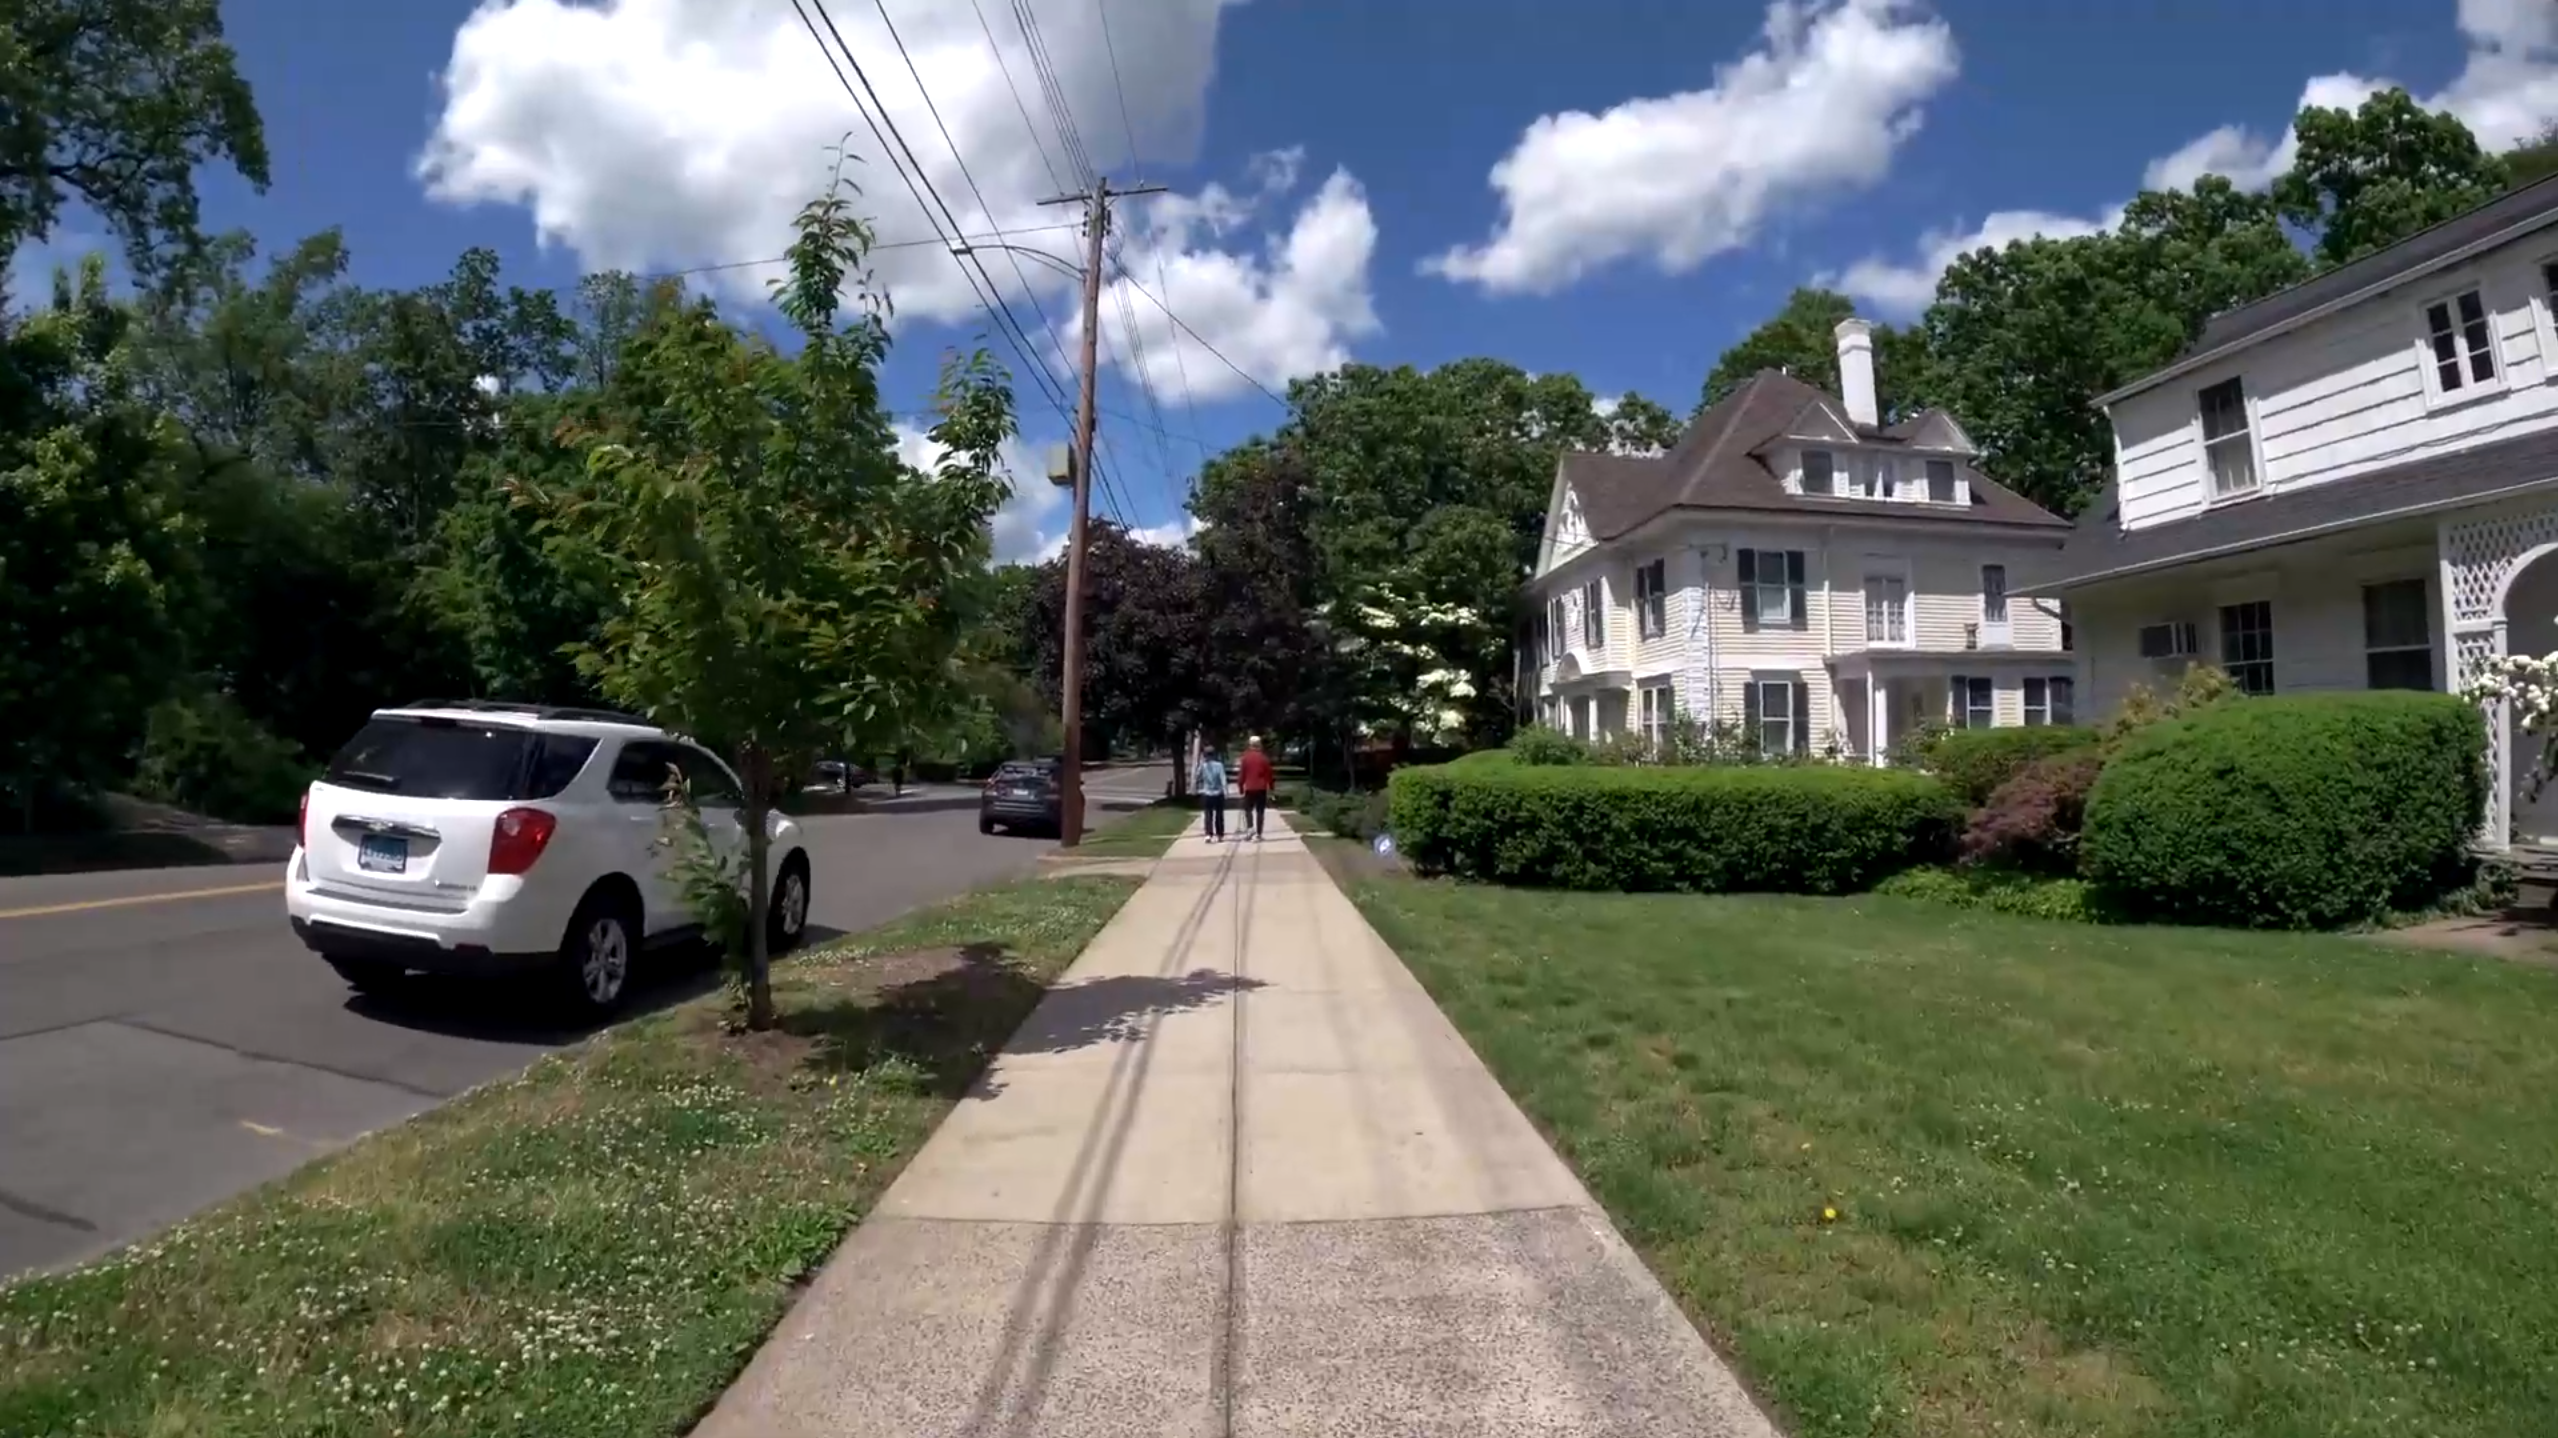
\includegraphics[width=0.80\textwidth]{screen_video_camminata}
\caption{Frame rappresentativo della sequenza di test: scena stradale con profondità prospettica, marciapiede convergente e oggetti a distanze variabili. Il movimento forward e le oscillazioni verticali legate ai passi costituiscono le perturbazioni principali da stabilizzare.}
\label{fig:screen_camminata}
\end{figure}

La scena presenta profondità prospettica con un marciapiede convergente, oggetti a distanze variabili e oscillazioni verticali ad alta frequenza sovrapposte al moto forward. Questo scenario è particolarmente adatto a evidenziare differenze tra modelli di trasformazione di complessità crescente.

Tutti i metodi sono stati eseguiti con \texttt{smoothing\_window}~=~45 e filtro gaussiano ($\sigma=2$), garantendo piena comparabilità dei risultati.

\section{Metriche di Valutazione}

Le prestazioni sono state misurate con:

\begin{itemize}
    \item \textbf{RMS} del moto incrementale su X, Y e rotazione (quantifica l'ampiezza del moto residuo),
    \item \textbf{Jitter Reduction (JR)} percentuale calcolata come riduzione della varianza degli step incrementali,
    \item \textbf{Tempo totale di elaborazione} (secondi, include solo i passaggi computazionali).
\end{itemize}

\[
RMS_x = \sqrt{\frac{1}{N-1}\sum_{t=2}^{N}(\Delta X_t)^2}, \qquad
JR_x = \left(1 - \frac{\mathrm{Var}(\Delta\tilde{X})}{\mathrm{Var}(\Delta X)}\right)\times 100\%
\]

\section{Risultati Quantitativi}

\begin{table}[H]
\centering
\begin{tabular}{lccccccc}
\toprule
Metodo & RMS X & RMS Y & RMS $\theta$ & JR X (\%) & JR Y (\%) & JR $\theta$ (\%) & Tempo (s) \\
\midrule
Block Matching        & \textbf{4.06} & \textbf{3.48} & --    & \textbf{97.4} & \textbf{94.9} & --    & 4843 \\
Opt.\ Partial         & 6.63 & 5.51 & 0.173 & 81.0 & 91.5 & 94.3 & 30.1 \\
Opt.\ Affine          & 6.53 & 5.85 & 0.173 & 84.5 & 90.8 & 95.8 & 30.1 \\
Opt.\ Homography      & 7.11 & 6.11 & 0.191 & 67.3 & 84.2 & 89.0 & 31.0 \\
ORB Partial           & \textbf{5.33} & 5.82 & 0.175 & 84.5 & \textbf{91.9} & 95.2 & 45.1 \\
ORB Affine            & 5.65 & 6.01 & 0.178 & 82.7 & 90.2 & 95.0 & 80.8 \\
ORB Homography        & 7.89 & 6.53 & 0.201 & 66.7 & 81.0 & 87.2 & 65.0 \\
\bottomrule
\end{tabular}
\caption{Confronto quantitativo tra tutti i metodi (\texttt{smoothing\_window}~=~45, filtro gaussiano $\sigma=2$). Block Matching non stima la componente rotazionale ($\theta$). In grassetto i valori migliori per ciascuna colonna (escluso Block Matching per il tempo, che impiega circa 4843\,s per via della ricerca esaustiva a grid)}
\label{tab:risultati}
\end{table}

\begin{figure}[H]
\centering
\includegraphics[width=\textwidth]{tabella_riepilogativa}
\caption{Tabella riepilogativa generata dall'interfaccia applicativa. I valori di Block Matching (JR~$>$~97\%) vanno letti con cautela: come mostrato dall'analisi delle traiettorie, il metodo stima moti nell'ordine di 100\,px cumulativi contro i $\sim$2500\,px di Optical Flow, indicando che il drift globale della camminata non viene stimato né compensato. Le metriche eccellenti di Block Matching riflettono la coerenza interna di una stima a corto raggio, non la qualità percettiva del video stabilizzato.}
\label{fig:tabella_riepilogativa}
\end{figure}

\section{Analisi delle Traiettorie}

Le figure seguenti mostrano le traiettorie cumulative lungo gli assi X e Y: la curva blu rappresenta il moto raw stimato frame per frame, mentre la curva arancione rappresenta il segnale filtrato (smoothed). La differenza tra le due curve è il contributo di compensazione applicato a ciascun frame.

\subsection{Block Matching}

\begin{figure}[H]
\centering
\includegraphics[width=0.9\textwidth]{traiettoria_block_matching}
\caption{Traiettorie cumulative X e Y -- Block Matching. I displacement massimi sono dell'ordine di 100\,px su X e 250\,px su Y: valori di gran lunga inferiori a quelli stimati dai metodi feature-based ($\sim$2500\,px su X per Optical Flow). Questo non indica maggiore stabilità, bensì la limitazione della ricerca a blocchi a corto raggio: il drift globale della camminata non viene catturato, e le metriche RMS/JR eccellenti riflettono la coerenza interna di una stima incompleta, non la qualità percettiva del video prodotto.}
\label{fig:traj_bm}
\end{figure}

\subsection{Optical Flow – Partial}

\begin{figure}[H]
\centering
\includegraphics[width=0.9\textwidth]{traiettoria_opt_partial}
\caption{Traiettorie cumulative X e Y -- Optical Flow Partial (Shi-Tomasi + LK). Il segnale filtrato insegue il drift forward lungo X preservando la stabilità verticale. Con RMS\,X~=~6.63\,px e JR\,Y~=~91.5\%, questo metodo offre il miglior compromesso tra qualità di stabilizzazione e velocità (30.1\,s).}
\label{fig:traj_opt_partial}
\end{figure}

\subsection{Optical Flow – Affine}

\begin{figure}[H]
\centering
\includegraphics[width=0.9\textwidth]{traiettoria_opt_affine}
\caption{Traiettorie cumulative X e Y -- Optical Flow Affine. Il modello affine introduce lieve miglioramento su JR\,X (84.5\% vs 81.0\% del Partial), ma incrementa RMS\,Y da 5.51 a 5.85\,px. La maggiore flessibilità del modello non si traduce in benefici sostanziali per questa tipologia di moto.}
\label{fig:traj_opt_affine}
\end{figure}

\subsection{Optical Flow – Homography}

\begin{figure}[H]
\centering
\includegraphics[width=0.9\textwidth]{traiettoria_opt_homo}
\caption{Traiettorie cumulative X e Y -- Optical Flow Homography. La traiettoria presenta oscillazioni più marcate rispetto al modello Partial: RMS\,X~=~7.11\,px e JR\,X~=~67.3\%, i valori più bassi tra le varianti Optical Flow. La proiettività amplifica gli outlier di matching in assenza di variazioni prospettiche reali.}
\label{fig:traj_opt_homo}
\end{figure}

\subsection{ORB Matching – Partial}

\begin{figure}[H]
\centering
\includegraphics[width=0.9\textwidth]{traiettoria_orb_partial}
\caption{Traiettorie cumulative X e Y -- ORB Partial. Il descrittore binario ORB consente una stima del moto traslazionale più precisa: RMS\,X~=~5.33\,px (il più basso tra i metodi feature-based) e JR\,Y~=~91.9\%. È il metodo a massima qualità tra quelli con tempi di elaborazione ragionevoli (45.1\,s).}
\label{fig:traj_orb_partial}
\end{figure}

\subsection{ORB Matching – Affine}

\begin{figure}[H]
\centering
\includegraphics[width=0.9\textwidth]{traiettoria_orb_affine}
\caption{Traiettorie cumulative X e Y -- ORB Affine. Il modello affine aumenta sensibilmente il tempo di elaborazione (80.8\,s, il più lento tra i metodi feature-based) senza migliorare le metriche rispetto a ORB Partial. RMS\,X~=~5.65\,px e JR\,X~=~82.7\% sono inferiori ai valori del modello Partial.}
\label{fig:traj_orb_affine}
\end{figure}

\subsection{ORB Matching – Homography}

\begin{figure}[H]
\centering
\includegraphics[width=0.9\textwidth]{traiettoria_orb_homo}
\caption{Traiettorie cumulative X e Y -- ORB Homography. La matrice omografica a 8 parametri produce i risultati peggiori nella famiglia ORB: RMS\,X~=~7.89\,px e JR\,X~=~66.7\%. Il matching ORB con omografia è particolarmente suscettibile agli outlier proiettivi in scene planari con moto prevalentemente traslazionale.}
\label{fig:traj_orb_homo}
\end{figure}

\section{Grafici Comparativi}

\begin{figure}[H]
\centering
\includegraphics[width=\textwidth]{grafici_comparativi_1}
\caption{Grafici comparativi (Parte~1): confronto tra metodi per RMS\,X, RMS\,Y e RMS\,$\theta$. I valori di Block Matching ($\approx$4\,px su X, $\approx$3.5\,px su Y) appaiono i migliori in assoluto, ma questo dato va interpretato con cautela: come evidenziato dall'analisi delle traiettorie (Figure~\ref{fig:traj_bm} e~\ref{fig:traj_opt_partial}), Block Matching stima un moto cumulativo di soli $\sim$100\,px contro i $\sim$2500\,px di Optical Flow. Le metriche RMS eccellenti riflettono dunque la \emph{scala ridotta} del moto stimato, non la qualità del video prodotto. I valori dei metodi feature-based (Optical e ORB) sono invece comparabili tra loro e rappresentano una misura affidabile del jitter residuo reale.}
\label{fig:grafici_comp_1}
\end{figure}

\begin{figure}[H]
\centering
\includegraphics[width=\textwidth]{grafici_comparativi_2}
\caption{Grafici comparativi (Parte~2): confronto tra metodi per Jitter Reduction percentuale su X, Y e $\theta$, e tempo di elaborazione. La JR di Block Matching ($>$97\%) è concettualmente non confrontabile con quella dei metodi feature-based: Block Matching riduce quasi interamente il poco moto che riesce a stimare, ma lascia il drift globale della camminata invariato, producendo un video percettivamente instabile. Il confronto significativo è quindi solo tra i metodi feature-based: ORB Partial e Optical Partial/Affine guidano con JR $>$80\% su entrambi gli assi, mentre le varianti Homography risultano sistematicamente inferiori. Sul piano del tempo, Block Matching è fuori scala ($\approx$4843\,s); tra i metodi feature-based Optical (30\,s) è circa il 50\% più veloce di ORB (45--81\,s).}
\label{fig:grafici_comp_2}
\end{figure}

\section{Discussione dei Risultati}

\subsection{Limiti delle metriche quantitative: il caso Block Matching}

Un confronto diretto tra le traiettorie di Block Matching e Optical Flow rivela una differenza concettuale fondamentale che le sole metriche numeriche non catturano.

La traiettoria di \textbf{Block Matching} (Figura~\ref{fig:traj_bm}) mostra un displacement cumulativo massimo di circa 100\,px su X e 250\,px su Y. La curva raw presenta oscillazioni visibili attorno alla tendenza generale, e la curva smoothed le segue con profilo attenuato -- le due curve sono distinguibili ma entrambe rimangono confinate in un range di spostamento molto limitato rispetto ai metodi feature-based. La traiettoria di \textbf{Optical Flow Partial} (Figura~\ref{fig:traj_opt_partial}), invece, raggiunge circa $-2500$\,px su X e $-800$\,px su Y: lo smoothing segue fedelmente il drift globale rimuovendo le oscillazioni ad alta frequenza.

Questa differenza non riflette una maggiore stabilità del video prodotto da Block Matching, bensì una \textbf{stima del moto incompleta}: la ricerca a blocchi opera su una finestra di ricerca limitata e stima solo traslazioni intere a corto raggio, rendendo invisibile il drift cumulativo della camminata. Di conseguenza:

\begin{itemize}
    \item il valore RMS calcolato è basso perché gli spostamenti stimati sono piccoli \emph{per costruzione}, non perché il video sia più stabile,
    \item la JR del 97\% rappresenta la riduzione del poco jitter che il metodo riesce a stimare, lasciando il moto globale sostanzialmente non compensato,
    \item il risultato visivo è un video che mantiene il drift della camminata, percepito dall'occhio umano come instabilità residua.
\end{itemize}

Optical Flow, stimando la traiettoria cumulativa reale, permette allo smoothing di applicare una compensazione ampia e continua. Il video stabilizzato risulta \textbf{percettivamente molto più stabile} nonostante le metriche numeriche (RMS e JR) siano inferiori a quelle di Block Matching.

Questo caso evidenzia un limite intrinseco delle metriche basate sul moto stimato: esse misurano la coerenza interna della stima, non la qualità percettiva della stabilizzazione. Un metodo che sottostima sistematicamente il moto reale può ottenere metriche eccellenti pur producendo un output visivamente inferiore.

\subsection{Optical Flow vs ORB}

A parità di modello di trasformazione (Partial), ORB fornisce un RMS\,X inferiore (5.33 vs 6.63\,px), confermando una stima del moto di base più precisa grazie ai descrittori binari. Optical Flow è invece più veloce (30.1 vs 45.1\,s), con un vantaggio di circa il 50\% sul tempo.

Per JR\,Y i due metodi sono sostanzialmente equivalenti (91.9\% vs 91.5\%), mentre ORB Partial supera Optical Partial su JR\,X (84.5\% vs 81.0\%).

La scelta tra le due famiglie dipende quindi dal vincolo applicativo: Optical Partial per il miglior compromesso qualità/tempo, ORB Partial per la massima stabilità. Entrambi stimano correttamente il moto globale cumulativo, garantendo una compensazione percettivamente efficace.

\subsection{Confronto tra Modelli di Trasformazione}

All'interno di entrambe le famiglie algoritmiche, il trend è coerente:

\begin{itemize}
    \item Partial $\geq$ Affine $>$ Homography in termini di JR e RMS,
    \item il tempo di elaborazione cresce con la complessità del modello,
    \item l'Homography penalizza sistematicamente le prestazioni di stabilizzazione.
\end{itemize}

Il modello Affine introduce parametri di scala differenziale e shear non necessari per descrivere le oscillazioni di camminata, risultando marginalmente peggiore rispetto al Partial. Il modello Homography (8 parametri) è chiaramente sovra-parametrizzato: amplifica gli outlier di matching proiettando errori locali in deformazioni geometriche globali (RMS\,X~=~7.89\,px per ORB Homography).

\subsection{Considerazioni sulla Sovra-Parametrizzazione}

I risultati confermano un principio generale: la complessità del modello deve essere commisurata alla natura del moto. Per una sequenza con moto forward costante e oscillazioni verticali periodiche, un modello a 4 parametri (traslazione + rotazione + scala isotropa) cattura il moto rilevante senza introdurre gradi di libertà instabili.

\section{Sintesi e Verdetto}

Escludendo Block Matching — le cui metriche numeriche eccellenti sono un artefatto della stima incompleta del moto, non una misura di qualità percettiva — \textbf{l'algoritmo migliore in assoluto per questa sequenza è ORB Partial}, con il miglior RMS\,X tra i metodi feature-based (5.33\,px) e la JR più alta su entrambi gli assi (84.5\% / 91.9\%) a fronte di un tempo di elaborazione accettabile (45.1\,s).

Se il vincolo è il tempo, \textbf{Optical Partial} rappresenta la scelta ottimale: produce una stabilità percettiva pressoché equivalente (JR 81.0\% / 91.5\%) in soli 30.1\,s, con un risparmio del 33\% rispetto a ORB Partial.

\begin{itemize}
    \item \textbf{Algoritmo migliore (qualità)}: \textbf{ORB Partial} — massima stabilità percettiva, stima del moto globale precisa, JR\,Y~=~91.9\%.
    \item \textbf{Algoritmo migliore (qualità/velocità)}: \textbf{Optical Partial} — risultato visivo equivalente a ORB Partial, 30.1\,s di elaborazione.
    \item \textbf{Da evitare}: varianti Homography (sovra-parametrizzazione, JR\,X $\leq$ 67\%) e Block Matching (stima del moto incompleta, risultato visivo inferiore nonostante JR numerica $>$97\%).
\end{itemize}

La lezione principale è che le metriche basate sulla stima del moto non sono sufficienti a valutare la qualità percettiva: occorre tenere conto della completezza della stima (copertura del moto reale) e non solo della sua coerenza interna.

% =================================================
% CAPITOLO 8 – Conclusioni
% =================================================

\chapter{Conclusioni}

\section{Riepilogo del Lavoro}

Il progetto ha prodotto un sistema completo di stabilizzazione video digitale con architettura modulare a cinque livelli. Sono stati implementati e integrati:

\begin{itemize}
    \item \textbf{Block Matching} con metrica SAD/MAD, eliminazione outlier via z-score e aggregazione configurabile (mediana, media, media pesata per confidenza);
    \item \textbf{Optical Flow} con rilevamento Shi-Tomasi, tracciamento Lucas-Kanade piramidale e stima della trasformazione (Partial/Affine/Homography) tramite RANSAC;
    \item \textbf{ORB Feature Matching} con Brute-Force Matcher, Hamming distance e Lowe's ratio test, abbinato agli stessi tre modelli RANSAC;
    \item tre filtri di smoothing della traiettoria (Moving Average, Gaussiano, Esponenziale IIR) con clamping automatico della finestra;
    \item compensazione geometrica con \texttt{warpAffine}, gestione bordi configurabile e cropping adattivo.
\end{itemize}

Il sistema espone le proprie funzionalità tramite un'interfaccia Streamlit con tre tab: stabilizzazione singola, confronto multi-metodo con barre di progresso dedicate, e analisi quantitativa delle metriche con grafici comparativi.

\section{Risultati Principali}

I test sperimentali su una sequenza di camminata a 1080p/30fps hanno prodotto i seguenti risultati chiave:

\begin{itemize}
    \item \textbf{ORB Partial} ottiene la stabilizzazione più efficace: JR X=87.7\%, JR Y=92.8\%, JR $\theta$=96.1\%, RMS X=5.16\,px, con un tempo di elaborazione di 24.9\,s.
    \item \textbf{Optical Flow Partial} offre un compromesso favorevole: elaborazione in 18.1\,s con JR~$\approx$~57\% su entrambi gli assi (configurazione con finestra 15 frame).
    \item Il modello \textbf{Homography} si rivela sistematicamente peggiore per questo tipo di moto, con RMS e JR inferiori rispetto a Partial e Affine in tutte le varianti testate.
    \item Il modello \textbf{Partial} (similitudine rigida, 4 parametri) è il più adatto a sequenze con moto prevalentemente traslazionale e oscillatorio, risultando più stabile numericamente rispetto ad Affine e Homography.
\end{itemize}

\section{Limitazioni del Sistema}

Il sistema presenta alcune limitazioni che ne circoscrivono l'applicabilità:

\begin{itemize}
    \item \textbf{Elaborazione offline}: la pipeline a due passate richiede l'intero video in ingresso; non è applicabile in tempo reale senza modifiche architetturali significative.
    \item \textbf{Perdita di campo visivo}: il cropping introduce una riduzione del campo visivo proporzionale all'ampiezza delle oscillazioni; con moto molto ampio, il \texttt{crop\_ratio} deve essere ridotto ulteriormente.
    \item \textbf{Scene dinamiche}: oggetti in movimento indipendente nella scena (pedoni, veicoli) possono contaminare la stima del GMV; la rimozione outlier via z-score mitiga ma non elimina questo problema.
    \item \textbf{Block Matching}: il metodo è in stato di sviluppo per i test di confronto; la stima di rotazione è fissa a zero, limitando l'efficacia su scene con componenti rotazionali significative.
    \item \textbf{Smoothing window}: la scelta della finestra è critica e dipende dalla velocità del moto intenzionale; finestre troppo ampie possono cancellare movimenti legittimi come pan e tilt.
\end{itemize}

\section{Considerazioni Finali}

Il progetto dimostra come un approccio modulare, con chiara separazione tra stima del moto, filtraggio e compensazione, consenta di integrare e confrontare algoritmicamente strategie diverse senza modificare l'infrastruttura. La disponibilità di metriche quantitative oggettive (RMS e JR) ha permesso di evidenziare che la complessità del modello non corrisponde necessariamente a prestazioni migliori: per il tipo di moto analizzato, il modello più semplice (Partial) si è rivelato il più efficace.

Il lavoro integra in modo coerente aspetti di visione artificiale, elaborazione numerica di segnali, geometria proiettiva e ingegneria del software, fornendo una base estensibile per applicazioni pratiche di stabilizzazione video.


% -------------------------------------------------
% Appendici
% -------------------------------------------------
% =================================================
% APPENDICI
% =================================================

\appendix

\chapter{Struttura Completa del Progetto}

\begin{verbatim}
src/
    motion_estimation.py     # MotionEstimator (Block Matching SAD/MAD)
    global_motion.py         # GlobalMotionEstimator (aggregazione, z-score)
    trajectory_smoothing.py  # TrajectoryFilter (MA, Gaussian, Exponential)
    motion_compensation.py   # MotionCompensator (warpAffine, crop)
    video_stabilizer.py      # VideoStabilizer (pipeline a due passate)
ui/
    tab_1v1.py               # Tab stabilizzazione singola
    tab_process.py           # Tab confronto multi-metodo
    tab_metrics.py           # Tab analisi metriche
    stabilization.py         # Application Logic Layer
    plot_utils.py            # Grafici Matplotlib
    video_utils.py           # Video comparativi + FFmpeg H.264
    config_loader.py         # Caricamento YAML
    styles.py                # CSS Streamlit
config/
    config_block_matching.yaml
    config_optical_flow.yaml
    config_orb.yaml
app.py                       # Entry point Streamlit
main.py                      # Entry point CLI
requirements.txt
\end{verbatim}

\chapter{File di Configurazione YAML}

\section{\texttt{config\_block\_matching.yaml}}

\begin{lstlisting}[language=bash, caption={Configurazione Block Matching}, basicstyle=\ttfamily\normalsize]
motion_estimation:
  block_size: 32          # Dimensione blocco (px)
  search_range: 12        # Raggio area di ricerca (px)
  metric: "sad"           # 'sad' o 'mad'

global_motion:
  motion_model: "translation"
  outlier_threshold: 2.0
  aggregation_method: "median"
  estimate_rotation: true
  estimation_method: "block_matching"

trajectory_smoothing:
  smoothing_window: 45
  filter_type: "gaussian"
  gaussian_sigma: 2.0
  exponential_alpha: 0.9
  deadband_px: 0.0

motion_compensation:
  crop_ratio: 0.85
  border_mode: "replicate"
\end{lstlisting}

\clearpage
\section{\texttt{config\_optical\_flow.yaml}}

\begin{lstlisting}[language=bash, caption={Configurazione Optical Flow -- Shi-Tomasi + Lucas-Kanade}, basicstyle=\ttfamily\normalsize]
global_motion:
  motion_model: "translation"
  estimation_method: "optical_flow"
  optical_flow:
    feature_type: "shi_tomasi"   # Shi-Tomasi corner detection + LK tracking
    transform_type: "partial"    # 'partial', 'affine', 'homography'

    # Shi-Tomasi + Lucas-Kanade
    max_corners: 1500
    quality_level: 0.002
    min_distance: 10
    block_size: 7
    win_size: 21
    max_level: 3

    # RANSAC
    ransac_reproj_threshold: 6.0

trajectory_smoothing:
  smoothing_window: 45
  filter_type: "gaussian"
  gaussian_sigma: 2.0
  deadband_px: 0.0

motion_compensation:
  crop_ratio: 0.85
  border_mode: "replicate"
\end{lstlisting}

\clearpage
\section{\texttt{config\_orb.yaml}}

\begin{lstlisting}[language=bash, caption={Configurazione ORB -- Oriented FAST and Rotated BRIEF}, basicstyle=\ttfamily\normalsize]
global_motion:
  motion_model: "translation"
  estimation_method: "optical_flow"  # pipeline condivisa, feature_type='orb'
  optical_flow:
    feature_type: "orb"          # ORB descriptor + BFMatcher Hamming
    transform_type: "partial"    # 'partial', 'affine', 'homography'

    # ORB
    orb_n_features: 1000
    orb_scale_factor: 1.2
    orb_n_levels: 10
    orb_edge_threshold: 31
    orb_ratio_threshold: 0.75    # Lowe's ratio test

    # RANSAC
    ransac_reproj_threshold: 6.0

trajectory_smoothing:
  smoothing_window: 45
  filter_type: "gaussian"
  gaussian_sigma: 2.0
  deadband_px: 0.0

motion_compensation:
  crop_ratio: 0.85
  border_mode: "replicate"
\end{lstlisting}


% -------------------------------------------------
% Bibliografia
% -------------------------------------------------
\bibliographystyle{plainnat}
\bibliography{bibliografia}

\end{document}
